\section{Implementation}\label{s:impl}
\begin{figure*}
    \centering
    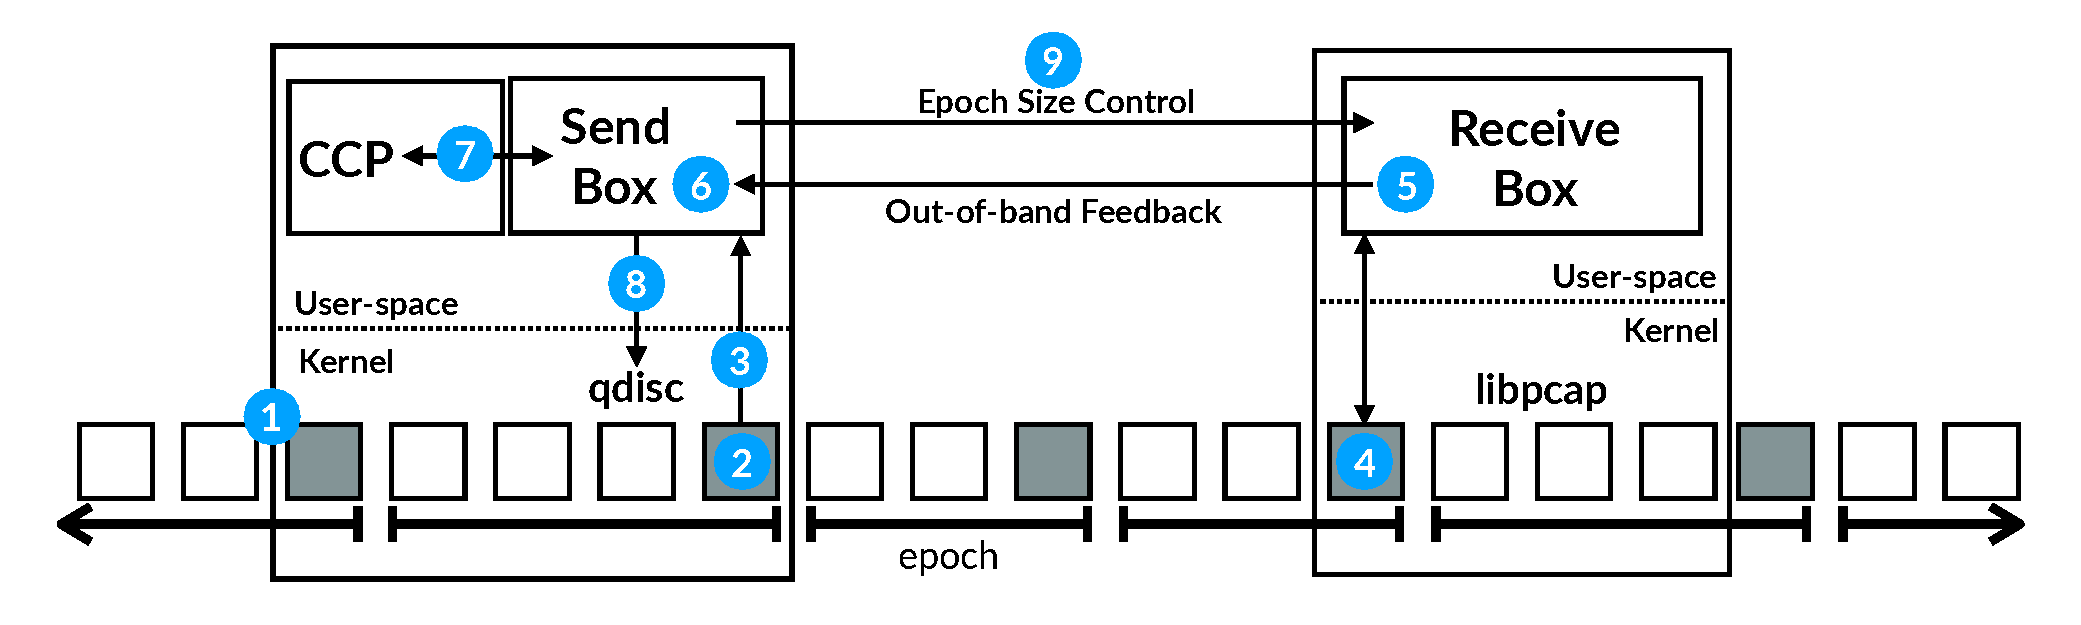
\includegraphics[width=2\columnwidth]{img/bundler-diagram}
    \caption{\name System Design
    \fc{add a separate line showing the epoch update from inbox to outbox}
    }\label{fig:bundler}
\end{figure*}

\cut{The prevalence of middleboxes today means that there are multiple options for implementing a \name \radhika{cut this line?}.}
We envision a two-part design for the \inbox: a ``control plane'' and ``data plane'' separation.
The data plane is responsible for packet forwarding, maintaining a count of the \cut{in-bundle} bytes sent, enforcing a rate and scheduling policy on the bundle, and reporting epoch boundary packets to the control plane.
These operations can be implemented either in software, via modern platforms for network function virtualization~\cite{bess, click, mos, netbricks}, or in hardware via programmable switches~\cite{p4} \radhika{move to end, see comment at end of paragraph}.
The control plane is responsible for computing measurements by combining feedback from the data plane and \outbox, and running the congestion control logic necessary to pick the appropriate rate for each bundle.
The \outbox is simple and does not require a control plane; it simply must observe the packet stream, maintain a byte count, and send reports to the \inbox on observing epoch packets.
The \outbox can, therefore, be implemented entirely in hardware if necessary \radhika{cut}.
\radhika{We envision the control plane to be implemented in software, while the data plane can be implemented in...(the line you had before)}

\subsection{Prototype}\label{s:impl:prototype}
For our prototype, we implement the inbox data-plane using Linux \texttt{tc}~\cite{tc}, and we limit our implementations of scheduling policy to those already widely available in the Linux kernel.
We patch the TBF queueing discipline (qdisc)~\cite{tbf} to enforce rates, and modify its ``inner\_qdisc'' to use a qdisc that enforces some scheduling policy.
Our patch to the TBF qdisc comprises $112$ lines of C.
The patch adds the functionality to detect epoch boundary packets, transmit feedback to the control plane using a netlink socket, and adjust the internal scheduling policy. 
Additionally, we remove one line in the rate update to disable re-filling the token bucket on rate changes to prevent a penalty for frequent rate updates.

We implement the \inbox control plane to run in user-space in $1167$ lines of Rust. 
It uses \texttt{libnl} to communicate with the qdisc, and \texttt{libccp}~\cite{ccp} to communicate with the congestion control algorithm via Unix-domain sockets.
It maintains the congestion control state of each bundle, but does not maintain (or observe) per-flow state.
\radhika{no. of LoC for \inbox dataplane?}

We implement the \outbox using \texttt{libpcap} in $188$ lines of Rust. It listens for packets on the interface, checks for epoch packets, and sends the reports to the \inbox. It must maintain per-bundle counters (described in \S\ref{s:impl:discovery}).

\radhika{an experiment showing scalability of bundler implementation?}

\subsection{\name Event Loop}\label{s:impl:loop}
Figure~\ref{fig:bundler} overviews the operation of our \name implementation.

(1) Packets arriving at the \inbox are sent to the qdisc. Those that match a bundle are put into the proper queue, 
otherwise they are forwarded immediately. (2) The qdisc observes a packet that matches the epoch boundary
condition (\S\ref{s:measure:marking}). (3) It sends a netlink message to the \inbox process running in user-space, which records the packet
in its epoch data structure, then forwards the packet along. (4) The \outbox observes the same epoch boundary
packet. (5) It sends an out-of-band UDP message to the \inbox containing the hash of the packet and its current state. 
(6) The \inbox receives the UDP message, and uses it to calculate the epochs and measurements as described 
in \S\ref{s:measurement}.

(7) Asynchronously, the \inbox invokes the congestion control algorithm every $10$ms \fc{periodically, for our prototype we set it to be 10ms, cite ccp} via \texttt{libccp},
giving it a chance to observe any new measurements and change its behavior. (8) If it decides to update
the bundle rate or congestion window, the \inbox communicates this to the qdisc
using \texttt{libnl}. Since the qdisc only supports rate enforcement, if the algorithm
also uses a congestion window, the \inbox computes $\text{\emph{effective rate}} = \frac{\text{CWND}}{\text{RTT}}$
and sets the rate of the qdisc to the minimum of the explicit rate and this effective rate\fc{only bbr uses this, if we cut bbr, cut this setion too?}.
Upon receiving new RTT samples, the \inbox updates the effective rate, and updates the qdisc rate
if appropriate.

\radhika{i liked this subsection!}


\subsection{Congestion Control}\label{s:impl:cc}
We use existing implementations of congestion control algorithms on CCP~\cite{ccp}; since CCP algorithms are already designed to receive network feedback asynchronously, they are a natural choice for our epoch-based measurement architecture. \radhika{this sentence should comer earlier, maybe when you first mention ``control-plane'' at the beginning of Sec 5, especially since 5.2 mentions CCP and libccp.}

\an{move to earlier, maybe design:}
It is important to note that traditional loss-based congestion controllers (\ie Cubic~\cite{cubic}, NewReno~\cite{newreno}) are poor choices for \name. 
This is because they double-penalize component traffic for losses: first, in the reaction of the end-to-end congestion controller to the loss, and second in the reaction of the controller at \name.

\an{missing connection here}
%Therefore, for algorithms which observe loss (Nimbus and Copa), we configure them to ignore it; the end-to-end reaction to loss will modulate the offered load to be the fair share of the bottleneck.
%
Further, we make a useful distinction between two types of cross-traffic conditions \name will experience.
We consider \emph{elastic} cross traffic and \emph{inelastic} cross traffic.
Elastic cross traffic (\eg Cubic, NewReno) probes for bandwidth and fills buffers at the bottleneck; inelastic cross traffic (\eg short flows) has limited demand and does not fill buffers.

When cross traffic is inelastic, the queueing delays that \name encounters will be self-inflicted. In these scenarios, scaling back and adjusting the sending rate at \inbox will cause the bottleneck to shift and the queueing delays at the bottleneck to reduce.
In the presence of elastic cross traffic, however, congestion control algorithms \emph{must} push packets into the bottleneck queue to remain competitive~\cite{bbr, copa, nimbus}.
As a result, we expect \name's benefits to disappear, since it must relinquish control of the queues to the bottleneck link.

\radhika{if above parts are covered in Sec 3, add a backwards pointer, and start with the implementation details below.}

Recent work~\cite{copa, nimbus} has considered the problem of switching between modes to take advantage of low queueing delays when it is possible to do so, yet reacting to and competing fairly with elastic cross traffic when it present.
Unfortunately, it is not immediately clear how to determine \name's fair rate once we detect elastic cross traffic.
The number of individual component connections which are backlogged at any given time may vary, and determining which connections should count towards \name's aggregate fair share rate would thus require per-connection state \radhika{not super clear to me}.

We sidestep this issue with a simple, yet powerful, observation: rather than attempt to compete with elastic cross traffic, \name should \emph{get out of the way} of its component connections.
The end-to-end congestion controllers responsible for \name's component connections will then naturally compete with and achieve their fair rate against elastic cross traffic.

It is important to implement this approach carefully. 
Consider a naive implementation in which upon detecting elastic cross traffic, \name stopped pacing packets entirely.
This approach would be unable to detect when the elastic cross traffic subsided, since it yields all control over the network queues.

Thus, when \name's congestion control algorithm detects that the cross traffic is elastic, it uses a simple control rule: \texttt{rate <- observed\_receive\_rate * 1.25}. 
This control rule will rapidly grow the pacing rate at the \inbox until it stabilizes at 25\% above the offered load.
Then, using the elasticity detection mechanism described in prior work~\cite{nimbus}, \inbox can modulate the pacing rate to determine when to retake control of the queueing, and therefore the scheduling policy.

\an{move the elastic cross traffic comparison results here?} \radhika{no, add a forward pointer}

\subsection{Bundle Initialization}\label{s:impl:discovery}

One practical concern in a \name deployment is how the \inbox and \outbox discover each others' presence. Of course, it is always possible to statically configure an \inbox and \outbox; however, this may be impractical as they reside in different networks.
Rather, we propose a bootstrapping mechanism wherein \name forms aggregates in response to observed packets.
This mechanism classifies packets traversing the \inbox and \outbox as either non-bundled (should be transmitted immediately and not paced in the qdisc) or bundled in a given qdisc. Different bundles may have different rates; recent work~\cite{carousel, eifel} has shown it is possible to implement such multi-rate, multi-scheduler datapaths efficiently.

The \inbox first assumes that all packets which traverse it are not bundled.
The \outbox does one of two things for each potential epoch boundary packet:
\begin{enumerate}
    \item If the packet is in a known bundle, the \outbox sends a message to the corresponding \inbox.
    \item If the packet is not in a known bundle, the \outbox sends a message to the source IP address of that packet.
\end{enumerate}

The \inbox receives (and intercepts) the \outbox feedback.  
The \inbox at this time updates its flow tables to add the destination IP of the epoch boundary packet either to an existing bundle (in the case of a new flow from a previously-unseen source subnet joining a bundle) or instantiates a new bundle.
The \inbox then sends a response containing an epoch size to use and the hash of the epoch boundary packet.
The \outbox receives this message, initializes a byte counter for the newly discovered bundle, and remembers the \inbox IP address for future feedback. If there is no \inbox on the path, the packet will simply be ignored at its destination. 


